\documentclass[12pt,a4paper]{article}
\usepackage[brazil]{babel}
\usepackage[utf8]{inputenc}
\usepackage[T1]{fontenc}
\usepackage{graphicx} % para inserção de figuras


\author{Universidade Católica Dom Bosco \\ Computação Gráfica - Engenharia da Computação \\Uéliton Freitas}
\title{Lista de Exercícios III}
\begin{document}
\maketitle


\begin{enumerate}
	\item O que  é \textit{flat surface rendering}? Dê exemplos.

	\item Descreve o método \textit{Gouraud surface rendering}. Qual  é a vantagem frente ao \textit{flat surface rendering}.
	
	\item Calcule o vetor normal médio dos vetores (0,0,1), (0,1,0), (1,0,0).
	
	\item Considerando o método \textit{Gouraud surface rendering}, calcule a intensidadedo ponto 4 ($I_4$) que está em (25,15) utilizando o deslocamento vertical.
Considere que o ponto 2 está em (40,10) com intensidade $I_2$ = 0.8 e o
ponto 1 está em (10,40) intensidade de $I_1$ = 0.2.

	\begin{figure}[!h]
		\label{Fig:are}
			\begin{center}
			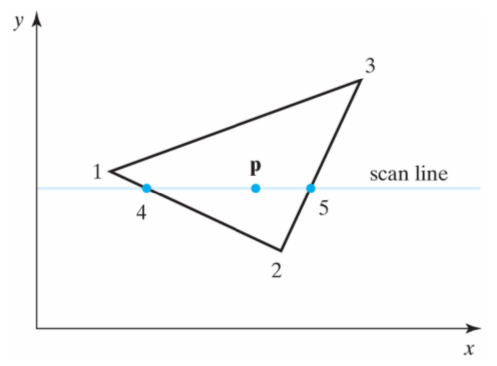
\includegraphics[width=0.48\textwidth]{PIC}
			\end{center}
	\end{figure}
	
	\item Descreva o algoritmo de \textit{Phong surface rendering}. Apresente três vantagens deste método de interpolação comparando-o com o \textit{Gouraud surface
rendering}. Qual é a sua desvantagem?

	\item Aplique o algoritmo \textit{Digital Differential Analyzer} (DDA) para fazer a coversã dos seguintes segmentos de retas:
		\begin{itemize}
			\item P1:(0,1) P2: (5,3)\\
			\item P1:(1,1) P2: (3,5)\\
		\end{itemize}
		
	\item Por que o DDA é considerado ineficiente?
	
	\item Qual é a vantagem do algoritmo de Bresenham quando comparado ao DDA?
	
	\item Aplique o algoritmo de Bresenham para o segmento de reta composta pelos pontos P1: (5,8) e P2: (9,11)
	
	\item Aplique o algoritmo de Bresenham para desenhar uma circunferência de raio 10 e centro na origem.
	
	\item Considere o polígono formado pelos pontos desenhados na ordem apresentada abaixo:\\
	
		p1 : (0,0,0)\\
		p2 : (10,0,0)\\
		p3 : (10,10,0)\\
		p4 : (5,8,0)\\
		p5 : (0,10,0)\\

		Identifique as arestas que fazem parte de uma concavidade neste polígono
utilizando produto vetorial.

	\item O que é necessário fazer para tornar este polígono concavo em um polígono
convexo.

	\item Execute o algoritmo apresentado em sala para converter um polígono em
uma malha de triângulo no polígono definido anteriormente.

	\item Explique a regra do par-impar para determinar uma região de interior e
exterior de objetos mais complexos.

	\item Porque o algoritmo \textit{scan-line} tem problemas ao passar por um vértices de exemplos.
	
	\item Como resolver o problema do \textit{scan-line} ao passar por um vértice?

\end{enumerate}


\end{document}